\documentclass[pageno]{jpaper}

%replace XXX with the submission number you are given from the ASPLOS submission site.
\newcommand{\asplossubmissionnumber}{XXX}

\usepackage[normalem]{ulem}
\usepackage{parskip}

\begin{document}

\title{\Large \bf Cyclone: Warp Speed Replication for Key Value Stores}


\date{}
\maketitle

\thispagestyle{empty}

\begin{abstract}
\vspace{0.1in}
Persistent key value stores are rapidly becoming an important component of many
distributed data serving solutions with innovations targeted at taking advantage
of growing flash speeds. Unfortunately their performance is hampered by the need
to maintain and replicate a write ahead log to guarantee availability in the
face of machine and storage failures. Cyclone is a replicated log plug-in for
key value stores that systematically addresses various sources of this
bottleneck. It uses a small amount of non-volatile memory directly addressable
by the CPU - such as in the form of NVDIMMs - to remove block oriented IO
devices such as SSDs from the critical path for appending to the log. It then
addresses network overheads using an implementation of the RAFT consensus
protocol that is designed around a userspace network stack to relieve the CPU of
the burden of data copies. Finally, it provides a way to efficiently map the
commutativity in key-value store APIs to the parallelism available in commodity
NICs via multiple transmit receive queues to scale replication performance on
multicore machines. Cyclone is able to replicate millions of small updates a
second using only commodity 10 gigabit ethernet adapters. As a practical
application, we use it to improve the performance and availability of RocksDB, a
popular persistent key value store by an order of magnitude when compared to its
own write ahead log without replication.
\end{abstract}

\section{Introduction}
Persistent key value stores are an increasingly important component of
datacenter scale storage services. Key value stores such as
Rocksdb~\cite{rocksdb}, LevelDB~\cite{leveldb} and FloDB~\cite{flodb} represent
large amounts of effort on both the engineering and research fronts. These key
value stores include sophisticated in-memory data structures built around Log
Structured Merge trees~\cite{lsmtree} and are heavily tuned to extract maximum
performance from flash-based solid state drives (SSDs).

These key value stores however tend to ignore an important component: the write
ahead log. A machine or storage failure leading to total loss or temporary
unavailability of data is unacceptable in services where high availabilty and
revenue are interconnected. Key value stores therefore usually incorporate
support for a write ahead log that if replicated and kept durable for every
appended update provides the necessary high availability. Unfortunately, the
write ahead log is a performance achilles heel for these systems - eclipsing
much of the work on improving the performance of the LSM component. To
illustrate the impact of the write ahead log, consider
Figure~\ref{fig:problem}. The line marked 'Rocksdb' shows the performance of
Rocksdb without the write ahead log. The performance when persisting the write
ahead log without replicating it is shown as the line marked 'rocksdb/WAL'. The
line marked 'rocksdb/3 way rep.' is for simply replicating the log three ways
without persisting it, using RAFT~\cite{raft} running over TCP/IP. Either
persisting every update to the log or replicating it using TCP/IP causes
performance to drop by an order of magnitude (note the log scale on the
x-axis). It is therefore no surprise that deployments of Rocksdb often turn off
the write ahead log~\cite{samza}. On the other side of the spectrum, key value
store research prototypes such as FloDB~\cite{flodb} turns off the write ahead
log to be able to showcase benefits of sophisticated extensions to LSM
datastructures.


\begin{figure}
\centering 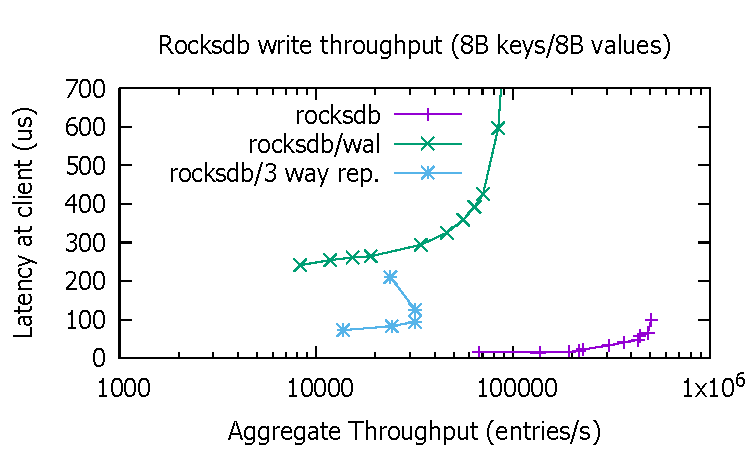
\includegraphics[scale=0.6]{results2/problem.pdf}
\caption{Rocksdb write ahead logging impact}
\label{fig:problem}
\end{figure}

Cyclone is a high speed strongly consistent replicated write ahead logging
service specialized for key value stores such as Rocksdb. Cyclone entirely
closes the performance gap due to both the storage and the network shown in
Figure~\ref{fig:problem}. We show that Cyclone achieves performance transparent
replication in that it can provide both a persistent write ahead log and
replication without compromising on RocksDB's performance.

The first key contribution of Cyclone is in showing how a small amount of
non-volatile memory can be combined with the flash SSD based persistent logs
when providing high availability.  The primary cause of slowdown when turning on
a write ahead log on a single machine in Figure~\ref{fig:problem} is the need to
do synchronous block IO for every update. For evenmoderately sized updates, this
leads to severe write amplification as a 4KB page must be synchronously written
to the log file on flash. Cyclone avoids this by making use of directly attached
persistent memory on the server. This can be in the form of NVDIMMs (DIMMs with
an added ultracapacitor to dump state to a small amount of attached flash) or
newer forms of persistent memory~\cite{pmfs}. For current deployments, NVDIMMs
are expensive - retailing at approximately 2X the price of a standard DIMM [find
  ref]. This means that they will likely be available in small quantities. We
compensate for this by periodically draining the NVDIMM log into a log placed on
a standard SSD on the system.

The second key contribution of this work is in showing that the performance
overheads in the network stack can be mitigated entirely in software. Existing
work on log replication using state machine replication protocols such as
Paxos~\cite{paxos} and RAFT~\cite{raft} has not - thus far - addressed high
performance replication in the local area network of a datacenter using
commodity networks.  Research focusing on addressing wide area network latencies
by reducing the number of network hops with new protocols such as Fast
Paxos~\cite{fast-paxos} or network switch modifications such as No
Paxos~\cite{nopaxos} do not address throughput bottlenecks due to network stack
related inefficiencies in the participating nodes of the quorum - a more urgent
problem with local area replication. On the other hand, work done to address
network related inefficiencies start with the assumption that the bottleneck to
good throughput on the network is the CPU and therefore one must either resort
to offload mechanisms such as RDMA~\cite{dare, farm, faast} or offload the
protocol entirely to an FPGA~\cite{consensus_box}. We demonstrate in this paper
that this is not the case. Rather, once persistence is provided by directly
attached non-volatile memory eliminating block IO from the persistence step in
replication protocols, the problem becomes equivalent to multicasting the same
log entry from the leader to all followers. We design Cyclone's network stack
around well known principles in the software packet switching community. In
particular, a careful implementation of a consensus protocol that relieves the
CPU of the responsibility of data movement permits a high performance
implementation entirely in software that addresses the order of magnitude
network related performance gap in Figure~\ref{fig:problem} using only commodity
10 Gigabit ethernet.

The rest of the paper is organized as follows. We describe Cyclone's system
architecture in Section~\ref{sec:sysarch}. We describe this two level log
structure in Section~\ref{sec:storage}. The set of optimizations to the network
stack is decribed in Section~\ref{sec:network}. Both the storage (NVM, SSD) as
well as the NIC expose significant parallelism that is left unused when Cyclone
is used to replicate a single log. To exploit this parallelism we use Cyclone to
replicate multiple logs, each using a different instance of the RAFT consensus
protocol. We show how to exploit the commutativity inherent in key-value store
interfaces to make use of this parallelism in Cyclone's design in
Section~\ref{sec:parallelism}.  A detailed evaluation of Cyclone's replication
is provided in the context of RocksDB - a popular persistent key value store -
in Section~\ref{sec:evaluation}. We then discuss related work before concluding.


\section{System Architecture}
\label{sec:sysarch}
A persistent key value store durably stores key-value mappings accessible through a
simple interface:

\begin{itemize}
\item GET(K): returns value corresponding to key K
\item PUT(K, V): sets the value of key K to value V
\end{itemize}

A key value store typically serves multiple client requests concurrently and is
linearizable~\cite{linearizability}. This means any history of requests and
responses can be rearranged such that responses immediately follow corresponding
requests and if a response precedes a request in the original history it also
does so in the rearranged history. Key value stores such as RocksDB also
support atomic writes to multiple keys and snapshots. 

Cyclone integrates with key value stores as both a client and server side
library. Cyclone replicates the key value store across a set of replica
servers. The client side library sends requests to a distinguished leader
replica.  On the server side Cyclone accepts requests from clients and calls
into the key value store. It then returns a response to the client. Before
executing any PUT request, Cyclone appends it to a durable log and replicates
the request to the logs of follower replicas. The request is considered
replicated once acknowledged by a majority of replicas.

Cyclone uses RAFT~\cite{raft} to keep the logs in sync across the replicas. On a
failure of the leader replica a new leader is automatically elected - RAFT
ensures that the new leader has the most up to date logs. The Cyclone client
library automatically locates the new leader on a failover - clients therefore
see only a brief interruption in service. Although read requests (GET
operations) are not logged, they are serviced in FIFO order with the write requests
(PUT operations) currently in Cyclone's log. This ensures linearizability in the
face of failovers.

\section{Storage}
\label{sec:storage}
Storage devices such as flash-based SSDs export a block IO interface. Appending
a small update to the write-ahead log requires a synchronous update of an entire
4KB page. This leads to a high baseline latency at even low load, as shown in
Figure~\ref{fig:problem}.  On the other hand small updates (in the order of 100s
of bytes for both the key and value taken together) are commonplace in many
workloads [find refs]. This problem leads many system designers to
underprovision key-value store shards ensuring that it operates at moderate to
high load, using group-commit to batch additions to the log. They therefore pay
a price in latency to ensure the bandwidth to storage is fully utilized to
prevent it from becoming a bottleneck.

Cyclone adopts a different strategy by making use of novel memory technologies
to obviate the need to make this tradeoff in the first place. We assume a small
amount of non-volatile memory directly addressable by the CPU rather than placed
behind a block oriented IO interface. Log appends are done to the ``NVM log''
placed in this non-volatile memory. While we designed Cyclone to leverage new
non-volatile memory technologies that might be available in the
future~\cite{3dxpoint} current non-volatile memory options such are NVDIMMs
are more expensive that DRAM. Therefore, for Cyclone to be economical
we cannot assume that a sufficient amount of NVM is available to hold the entire
log. The log entries can only be garbage collected when the in-memory component
of the key value store is checkpointed to secondary storage. The growing size of
available DRAM means that also provisioning sufficient NVDIMMs to hold the
corresponding log of updates is not feasible given that NVDIMMs cost at least
twice as much as volatile DRAM. We therefore resort to using a second larger log
level placed on a flash SSD. Entries are drained from the NVM log to this flash
log in conveniently large units that are a multiple of 4KB - the optimum IO unit
for flash SSDs. This ensures we get the best
possible throughput from a flash device without paying the price of synchronous
IO for small key-value pairs. At the same time, the amount of non-volatile
memory required is small enough to not add undue cost of the server.

The flashlog is written out in segments of configurable size (we use 128KB
segments). A segment buffer is prepared in memory (volatile DRAM) using the
layout shown in Figure~\ref{fig:flashlog_page}. We do not allow objects in the
flashlog to cross a 4KB boundary - linking multiple objects together with a
special flag encoded into the size if necessary. We flush log segments out to
the log file using asynchronous direct IO, and therefore we fill one log segment
buffer while keeping IO to another one outstanding to the flash drive. To avoid
having to do a synchronous metadata flush, we preallocate (using the
posix\_fallocate call) a gigabyte worth of zero filled disk pages at the end of
the log file whenever we hit its end.

In order to recover from a crash, we make two important assumptions about the
underlying SSD. First, we assume that 4KB is the \emph{minimum} atomic unit for
updating pages on the SSD even under power failure i.e. there are no shorn
writes (otherwise known as torn writes) on a 4KB page~\cite{shorn_writes}. We
also assume that the SSD has power loss data protection meaning that writes
cached in the drive's volatile cache are written to the SSD using a backup
capacitor in the event of power failure - a property of many data center class
SSDs today, including the Intel DC P3600 SSD~\cite{ssd_spec} we use in our
evaluation. Together these two assumptions mean that we can recover a consistent
prefix of the log on a power failure.

We move log entries from the head of the NVM log to the flashlog buffers in FIFO
order. The NVM log entry is only actually removed when the IO for the
corresponding flashlog page is complete. This means that during recovery we can
have the same log entry both in the NVM log and the flashlog, a condition that
can be detected by examining the log sequence number that we embed in each log
entry.

\begin{figure}
  \centering
  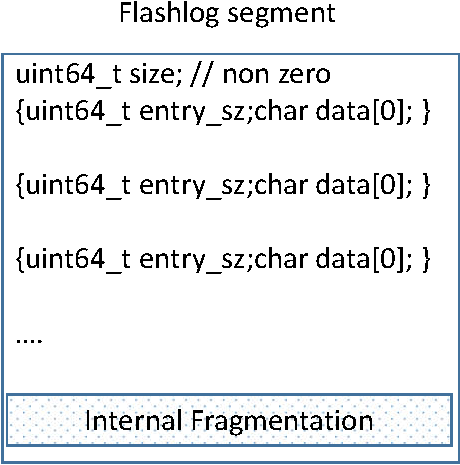
\includegraphics[scale=0.4]{figures2/flashlog_page.pdf}
  \caption{Flashlog segment}
  \label{fig:flashlog_page}
\end{figure}

The two level log design in Cyclone lays the foundation for improvements to the
network stack that we discuss next - a significant contributor to the overheads
in Figure~\ref{fig:problem}. We use RAFT to replicate the NVM log from the
leader replica to the followers. Each replica \emph{independently} drains
committed entries (in terms of RAFT consensus) from the NVM log to the
flashlog. Block IO therefore is no longer a consideration when optimizing data
movement over the network, unlike systems that need to deal with such
problems~\cite{reflex}. Replication reduces to efficiently sending a block of
data already present in directly attached memory over the network. 

\section{Network}
\label{sec:network}

The core network operation in replication is to receive a request from the
client at the leader replica and send that exact same request (as a log entry)
to all follower replicas. The leader therefore \emph{multicasts} a received
request packet to follower replicas, a problem well studied in the networking
community when building software packet switches. Software packet switches reach
impressive speeds of millions of packets forwarded per core [find refs], a
number far in excess of the few hundreds of packets we manage in
Figure~\ref{fig:problem}. We therefore proceed by approximating a software
packet switch for the networking component of Cyclone. However software packet
switching does not need to deal with failure - usually requiring only a simple
decision for each packet at the node. RAFT introduces significant
protocol level work for each forwarded packet a challenge that we need to deal
with to approach the desired software packet switching efficiency in the common
case.

\subsection{DPDK}
The Data Plane Development Kit~\cite{dpdk} provides low latency userspace access
to an ethernet NIC, permitting the application to directly send and receive raw
ethernet frames via the transmit and receive queues on the NIC. DPDK is often
used by developers of software packet switches and therefore we also leverage
DPDK as a library for building Cyclone.

DPDK does not by itself provide a TCP stack. This is not a problem. RAFT (and
indeed most consensus protocols) tolerate network losses and reordering by
design due to the need to support asynchronous communication. In addition, most
datacenter networks rarely drop or reorder packets and provide full bisection
bandwith between servers that might serve as Cyclone replicas. We therefore
jettisoned TCP and chose to send raw IP packets encapsulated in ethernet
frames. We currently follow this communication model both for server to server
communication between replicas as well as client server communication for
requests and responses. Although a detailed evaluation is made later, switching
from the kernel TCP/IP stack to DPDK reduces the latency between machines in our
testbed from {\tt 24 us} to as low as {\tt 5 us}, providing a significant boost
to performance.

We direct DPDK to use pages backed by NVM for packet buffers. DPDK uses a
concurrent memory allocator based on reference counting - used by both the NIC
driver and CPU cores. This means that packet allocation and deallocation does
not happen in the same order as their corresponding position in the replicated
RAFT log. To deal with this, we use a level of indirection as shown in
Figure~\ref{fig:nvm_log}. The NVM log is maintained as a circular log of fixed
sized pointers. Adding a level of indirection in the NVM log allows us to
separate the FIFO ordered circular log being manipulated by RAFT from packet
data being managed by the memory allocator of DPDK. Both the circular log and
packet data are in NVM. An advantage of this scheme is that it makes recovery
from NVM easy - appends to the circular pointer log are atomic and we can use
the pointer log to recover allocator state i.e. what pieces of NVM are currently
in use by the log.

\begin{figure}
\centering
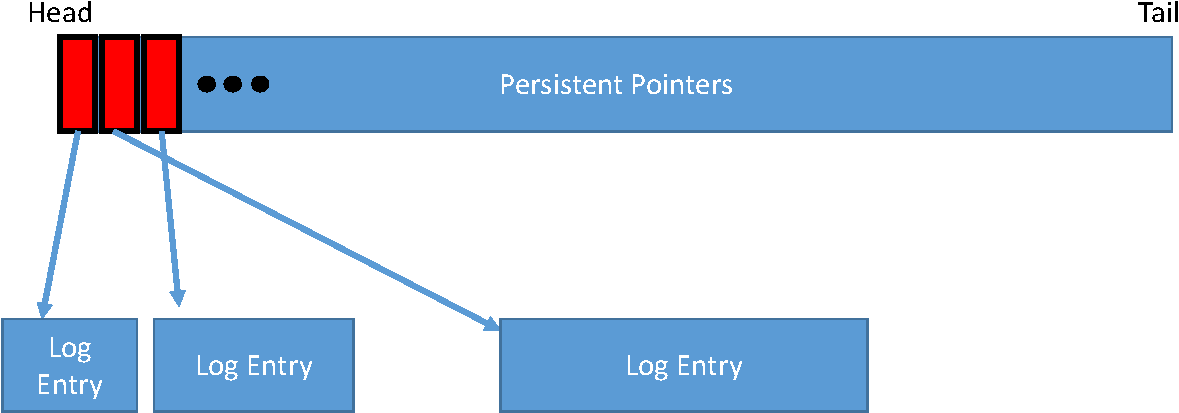
\includegraphics[scale=0.3]{figures2/nvm_log.pdf}
\caption{NVM log structure}
\label{fig:nvm_log}
\end{figure}

\subsection{Eliminating Data Movement}
Software packet switches built on DPDK try to touch as little of the packet data
as possible, minimizing movement of data up and down the cache and memory
hierarchy. Log replication looks like multicast that does not require deep
packet inspection. Software packet switches implementing multicast therefore
simply manipulate packet headers to produce new packets to send on the output
ports. We designed our implementation of raft around the same principle.

\begin{figure}
\begin{verbatim}
    event_receive_client_req()
    {
      if(!check_is_leader()) {
        drop_msg
        return
      }
      Prepend raft log term and index
      Persist to local log
      Transmit to follower replicas
    }
\end{verbatim}
\caption{Cyclone event handling}
\label{fig:control_plane}
\end{figure}


The pseudocode in Figure~\ref{fig:control_plane} describes part of the packet
handling code in Cyclone organized as event handlers triggered on receiving a
packet at the leader. We focus on only one key event for brevity: the event
where a request is received from a client. The first step is to check that this
replica is indeed the RAFT leader in the current view (term). If not, the
message is simply dropped (a timeout causes the client to try a different
server). It then prepends RAFT related information to the packet - this includes
the current term and log index for this entry. Next, it appends a pointer to the
log in Figure~\ref{fig:nvm_log} effectively appending the packet to the
persistent log. Finally, it transmits the packet to follower replicas.

This entire process is done without making any copies of the received packet.
To illustrate how this is achieved, Figure~\ref{fig:packet_layout} shows how
Cyclone manipulates packet
layouts across the two steps of prepending a RAFT header and transmitting to
follower replicas. DPDK describes packets using an ``mbuf'' data
structure. Roughly speaking, an ``mbuf'' consists of a flat array of bytes
actually containing the packet and a fixed size piece of external metadata that
describes various aspects of the packet, most crucially a pointer to the start
and end of the packet in the byte array. DPDK's userspace drivers receive
packets from the NIC such that they are offset in the byte array by a
configurable amount referred to as ``headroom''. We strip off the existing
network headers in the packet and prepend RAFT related information specific to
each log entry in the headroom by shifting the start pointer appropriately.
These operations are standard enough for software packet switches that DPDK
provides convenient library calls for it. For the final step, we need to prepare
the packet for transmission to the various follower replicas. To do this we
prepare a different packet containing an ethernet header for \emph{each}
targeted replica and ``chain'' the data packet to each of these headers. Each
header is then separately handed off to the driver for transmission via the NIC,
carrying the data packet with it by association.

\begin{figure}
  \centering
  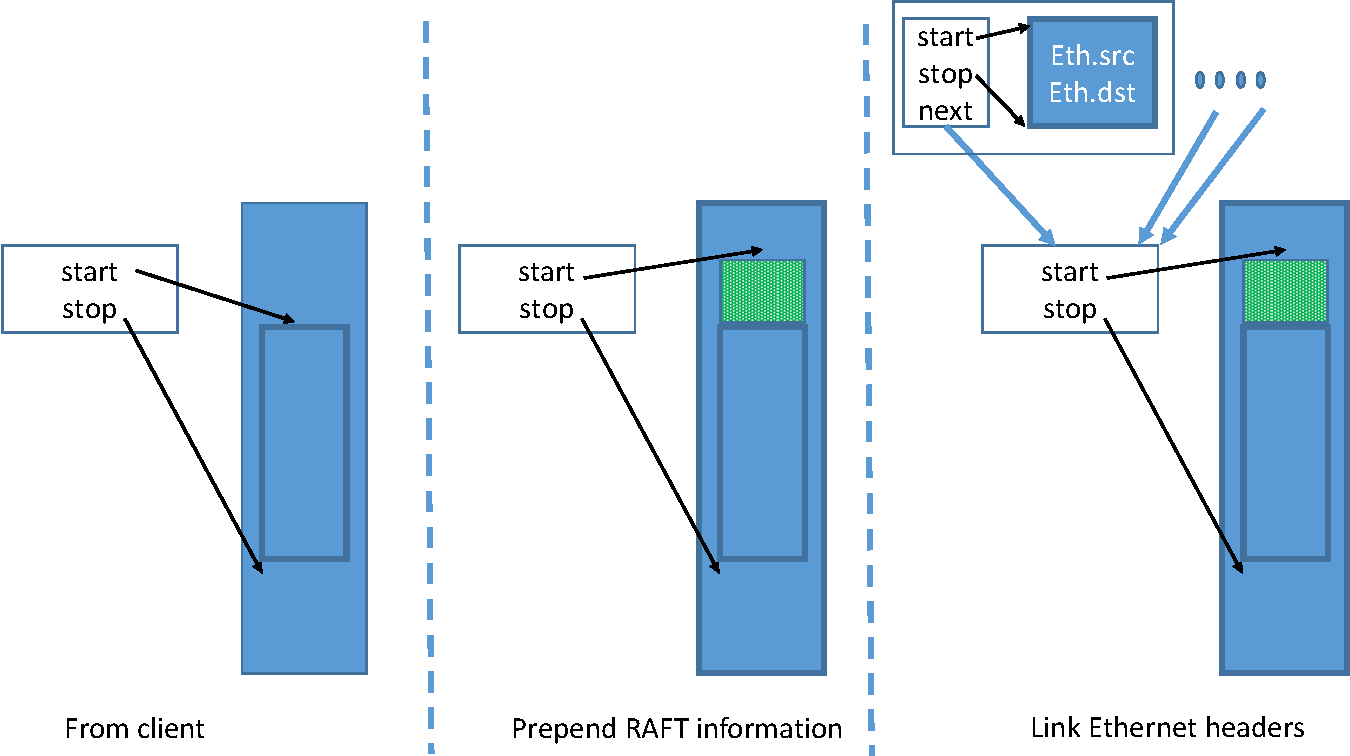
\includegraphics[scale=0.35]{figures2/network_packet.pdf}
  \caption{Cyclone network packet layout}
  \label{fig:packet_layout}
\end{figure}

We now turn our attention to the persistence step in
Figure~\ref{fig:control_plane}. RAFT requires that the log entry be persisted
before it is multicast out to follower replicas. DPDK userspace NIC drivers
operate in DDIO mode~\cite{ddio} where the packet is directly written into the
CPU cache rather than first being DMAed into DRAM and then fetched by the CPU on
demand. Since the NVM is directly attached we need to persist the packet to it
by executing a cacheline flush ({\tt clflush}) instruction for every cacheline
in the packet and the pointer in the pointer buffer to persist these via the
memory bus. This is not too onerous a burden because we can use the newly
introduced {\tt clflush-opt}~\cite{clflush_opt} instruction specifically
intended to efficiently flush to persistent memory without the overhead of the
serialization normally introduced by {\tt clflush}. This allows us to hit full
memory bandwidth on present generation platforms, a quantity in excess of 200
Gb/s per core, well above the near term speeds of network interface cards. We
execute a single serializing {\tt sfence} before the sequence of {\tt clflushes}
to make sure any dirty cacheline due to header manipulation related writes from
the CPU are sent to cache.

\begin{figure}
  \centering
  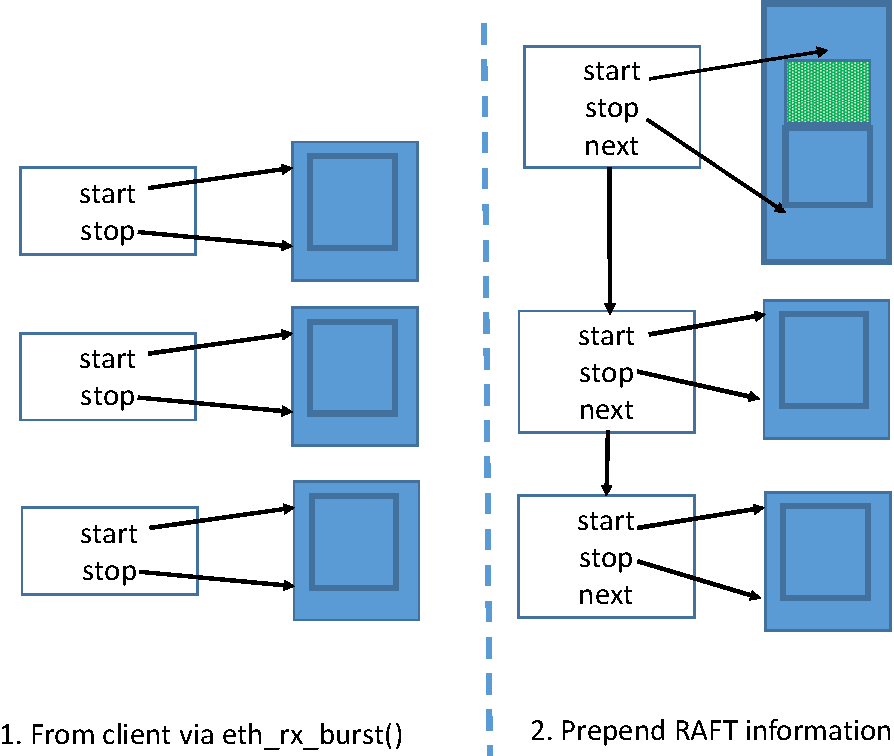
\includegraphics[scale=0.4]{figures2/batching.pdf}
  \caption{Batching}
  \label{fig:batching}
\end{figure}

Although RAFT is an efficient consensus protocol in the common case, the
protocol state machine still adds significant overhead to each packet, relative
to the time for the packet to flow in from the NIC and back out to the replicas.
We address this problem for the \emph{loaded} case using batching - treating a
whole sequence of client commands as a single RAFT log entry, while avoiding any
copies to group these packets together. Figure~\ref{fig:batching} illustrates
how this is done. We use a burst receive call available in the DPDK userspace
driver to receive a burst of client packets at a time. We then chain these
packets together and treat them as a single log entry from the perspective of
RAFT, amortizing the control plane overheads over the packets (at most 32 at a
time due to current driver limitations). Crucially, batching in Cyclone does not
involve a latency-throughput tradeoff like in many other
systems~\cite{ix-dataplane}. The batch receive call we use in DPDK returns
immediately with whatever number of packets is available, including zero. We
always flush the transmit buffer after every call to DPDK to transmit packets to
replicas. Therefore, we never tradeoff latency for throughput when batching. 


\section{Parallelism}
\label{sec:parallelism}

%\begin{figure}
%  \centering
%  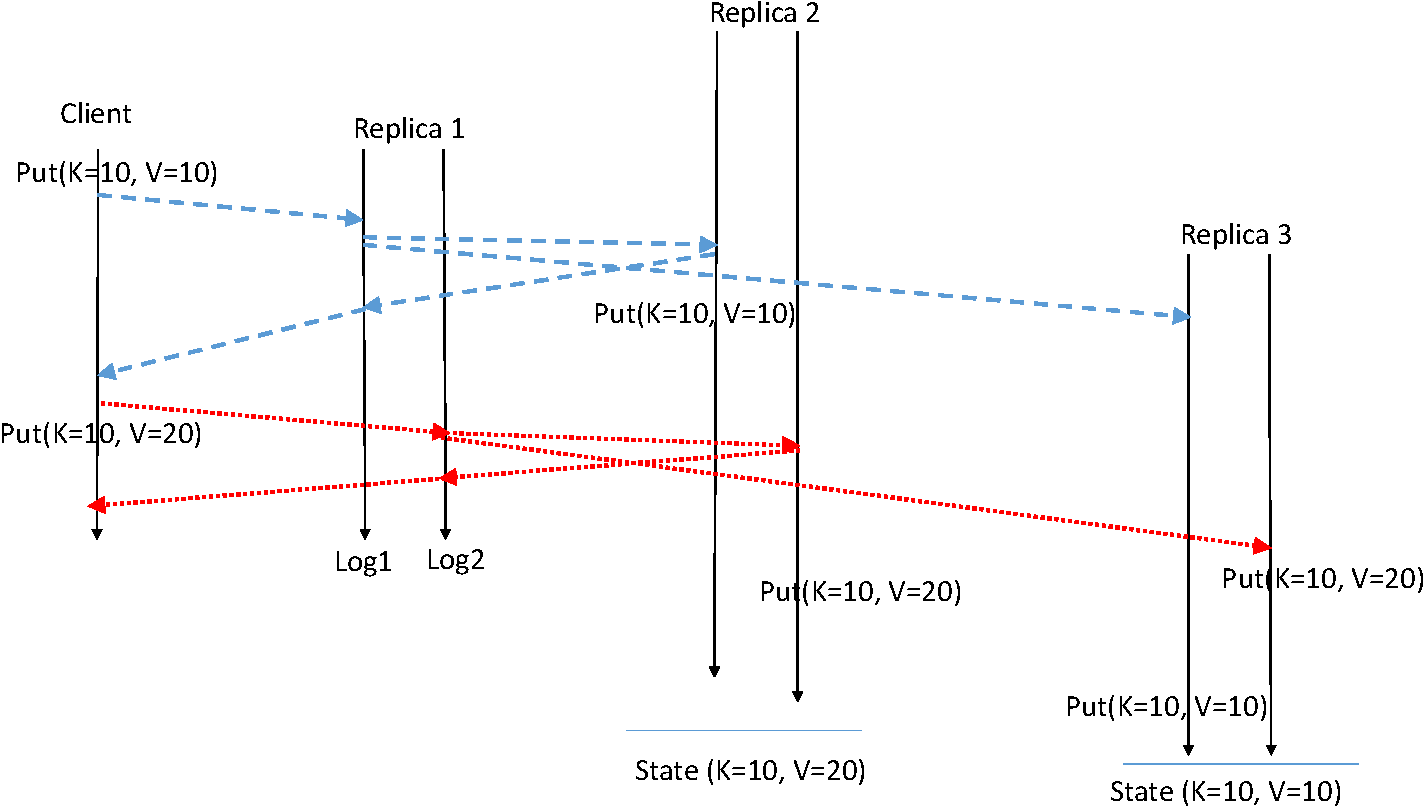
\includegraphics[scale=0.35]{figures2/race.pdf}
%  \caption{Race with multiple physical logs}
%  \label{fig:race}
%\end{figure}

Althought the work described in the previous section significantly boosts the
network performance of replication in Cyclone, it still does not come close to
saturating the capabilities of even the commodity network interface card that we
use. This is because NICs today encapsulate significant parallelism in terms of
multiple send and receive queue pairs. Exploiting this capability to improve
throughput requires us to remove the bottleneck of a single sequential log in
RAFT. To this end, we extend the implementation described thus far to run
multiple copies of the RAFT consensus protocol each maintaining and replicating
its own two level log. We now refer to these logs as physical logs. All these
instances however exist in the same process address space as the key value store
application itself and therefore manipulate the same application.


The first key question we deal with is - how do Cyclone clients decide which
physical log to send a {\tt PUT} or {\tt GET} request to ? A key constraint here
is that all replicas should agree on the seqeunce of updates to a key - as
otherwise they would diverge in terms of state. Allowing updates to the same key
to go to different physical logs would lead to a divergence as there is no
guarantee about the order in which the independent RAFT instances would apply
the update. Therefore all updates to a key must go to the same physcial
log. A similar constraint applies to reads in order to ensure that any committed
writes are seen by readers. Allowing reads to a key to go to a different RAFT
instance than the write means that it could be served on a machine where the
write is yet to be applied but where the machine is the leader for the RAFT
instance. All reads and write to a key must therefore go to the same physical
log. We achieve this by hashing the key to select the physical log.

It turns out that this simple \emph{necessary} scheme is also \emph{sufficient}
to ensure linearizability in the face of failure. Clearly the system is
linearizable for a single key since it involves only a single physical log. In
addition, one can switch operations to different keys in a history without
affecting the correctness of the history because operations to different keys
are commutative. Any history of the system is therefore linearizable.

Multiple physical logs in Cyclone operate in a shared nothing manner by
partitioning the NVM and SSD space evenly between them and by allocating
dedicated NIC queue pairs to each instance of RAFT. This works well because the
memory hierarchy including the NVM and the SSD efficiently support concurrent
operations. The only synchronization necessary is when doing reads or writes to
the single shared key value stores.  The level of concurrency therefore is
constrained only by the concurrency available in the software architecture of
the persistent key value store itself, for which a number of good designs
already exist~\cite{flodb}.

In our discussion thus far, we have focused on operations to a single
key. Supporting atomic writes or reads to multiple keys while maintaining
linearizability requires special handling with multiple physical logs so as not
to break linearizability - that we discuss next.

\subsection{Ganged Operations}
Supporting reads or writes to multiple keys that map to different physical logs
requires a ganged operation across those logs such that all the operations
complete together in the face of failures. Since our starting point is a single
key value store, we constrained Cyclone's design early on to avoid the need for
any two phase commit.

The first key problem we need to deal with is that the leaders for the different
RAFT instances can be located on different machines. To avoid having a client
co-ordinate different machines for a single operation, we constrain the RAFT
leader election algorithm for the different RAFT instances to converge to the
same machine. We do this by triggering re-elections for a RAFT instance other
than that of the first physical log until it is on the same machine as the
\emph{first} physical log. This process is therefore resilient to failed
machines. RAFT requires that the leader have the most up to date log. To ensure
that the process converges we therefore ensure that the currently elected leader
brings a majority quroum up to date before triggering a relection. We also do
not accept any requests from clients until all leaders are co-located. This
process is guaranteed to converge as long as all no network partitions occur
\emph{within a machine} i.e. some RAFT instances are able to send and receive
packets, while others are not, a possiblity we discount due to our single
process design.

Next, we need to simultaneously inject the ganged operation into all
participating physical logs on the machine hosting the leaders. Clients always
dispatch batched writes to a fixed co-ordinating physical log/RAFT instance
(henceforth called the co-ordinator), which is then responsible for forwarding
the request to the participating logs. We make use of packet cloning primitives
to avoid making a physical copy of the packet, generating indirect references
instead. The co-ordinator also adds a ``nonce'' - a unique timestamp to the
packet. In addition, the co-ordinator adds a unique view number to the packet
containing the term numbers of all the participating RAFT instances (read from
shared memory of the co-located leaders).  The event that applies a ganged
operation is described in the pseudocode of Figure~\ref{fig:ganged_ops}. We
defer the discussion of how we generate the nonce to later in this section. We
also assume that a unique barrier is allocated in shared memory for each ganged
operation. We discuss later how this is done without using dynamic allocation.

The complexity in Figure~\ref{fig:ganged_ops} arises from the need to handle
both shared memory concurrency and failure during replication. Without failure,
Figure~\ref{fig:ganged_ops} is straightforward. A barrier is executed on all
RAFT instances. Once replication is complete on all participating physical logs
(or this is a read ganged operation), a state indicated by all necessary bits
being set in the barrier mask, the RAFT instances simultaneously execute the
ganged operation.

Each RAFT instance always publishes the current term it is operating in. A
failure causes a new leader to be elected moving forward the term. If the
participants of a ganged operatation do not detect this case, they could be left
waiting for ever as ganged operation might never successfully replicate in the
failed over RAFT instance. We detect failure on any RAFT instance by having each
instance publish its current term and continuously comparing the view in the
ganged operation to it. If any RAFT instance has moved past that term, the
ganged operation is then terminated by having one of the still alive participants set a
failure flag and write the appropriate bit in the barrier mask on behalf of the
failed participant, moving execution past the barrier wait - a technique we
borrow from lock-free data structures~\cite{lock-free}.

\begin{figure*}
  \centering
\begin{verbatim}
    // Apply ganged operation
    event_apply_ganged_op (packet, barrier)
    {
      if(co-ordinator)
        atomic set bit me in barrier.mask         
        do
         for each participant p in operation
          if public_data[p].view > packet.view
           barrier.failed = true 
           atomic set bit for p in barrier.mask
        while barrrer.mask != mask of all participants
        if barrier.failed
         Ganged replication failed. Send retry to client. return.
        else       
         execute operation
         send response
      else
        wait until 
         public_data[co-ordinator].view > packet.view OR
         barrier.mask == mask of participating KV cores
        if public_data[co-ordinator].view > packet.view OR
           barrier.failed
         Ganged replication failed. Send retry to client. return.
        else
         execute operation
    }
\end{verbatim}
\caption{Ganged Operation}
\label{fig:ganged_ops}
\end{figure*}

The assumption in Figure~\ref{fig:ganged_ops} is that each ganged operation is
mapped to a unique barrier. We achieve this by using a fixed piece of memory
owned by the co-ordinator to hold the barrier and write the nonce to it in order
to indicate that the barrer is active for the corresponding ganged
operation. Participants watch for the nonce to know when to execute the
ganged operation barrier in Figure~\ref{fig:ganged_ops}, while also monitoring
the leader's published view to detect the case where the ganged operation fails
to replicate on the co-ordinator's physical log.

Finally, we describe how we generate the nonce. The nonce is generated on the
co-ordinator RAFT instance by concatenating the ethernet MAC ID of the first NIC
on the system with a 64 bit value that is the number of CPU timestamp counter
cycles since epoch time (read from the real time clock at startup plus the
number of cycles from the CPU {\tt rdtsc} instruction). The nonce can only be
repeated if the same machine manages to fail and come back up in less time than
the real time clock drift (controlled with NTP), a possibility that we discount.

Ganged operations possibly consititute the most complex part of Cyclone but the
code weighs in at well under a couple of hundred lines. We believe that
this additional complexity is still small compared to distributed transactions
using two-phase commit that also need to recover from failure used in systems
such as FARM~\cite{farm}.

\section{Evaluation}
\label{sec:evaluation}
We evaluate Cyclone on a 12 node x86 Xeon cluster connected via a 10 GigE
switch. Three of the machines are equipped with 1.6TB Intel DC P3600 SSDs and
4*10 GigE ports. The remaining nine machines do not have SSDs and have only one
10 GigE port, serving as clients for most of the experiments. We turn on jumbo
frame support in the 10 GigE switch to enable maximum use of batching in
Cyclone. As with other work~\cite{faast}, we use DRAM on the machines to proxy
for NVDIMMs where necessary - the persistent memory needed never exceeds 64 MB
regardless of the size of the key value store or second level log on flash. We
divide the evaluation into three parts. First, we evaluate Cyclone's performance
with a single level log as a pure software packet switch. Next, we evaluate
performance when adding a second level of log on flash. Finally, we evaluate
performance when integrated with Rocksdb~\cite{rocksdb} as an alternative to
Rocksdb's write ahead log. Unless otherwise mentioned, we use a 60 byte header
followed by an optional payload for experiments. We log both the header and
payload. In all cases the server echoes the received entry (header and payload)
back to the client. We fix the number of KV Store threads at 32 using at most 8
physcial logs with associated control plane cores for running RAFT instances.

Cyclone is built on top of DPDK to apply software packet switching techniques to
the log replication problem. We therefore begin by systematically evaluating
optimizations applied in Cyclone to replicate the NVM log in
Figure~\ref{fig:network_opts} - with no payload. The y-axis reports latency seen
at the client (which means two network round trips with replication). Using
TCP/IP to replicate a RAFT log tops out at around 30K entries/s.  Switching to
DPDK (the line marked +DPDK) improves the throughput by an order of magnitude to
around 500K entries/s. Using batching (the line marked +batching) improves the
performance further bringing us close to a million entries/s. Scaling
horizontally to 8 physical logs (+8 phy logs) improves performance to close to
2M entries/s. Finally using all 4 ethernet ports on the machine to replicate
entries improves performance considerably to 6M entries/s. In all, performance
improves by 200X over the TCP/IP single log baseline. Cyclone also considerably
improves the latency for replication, from close to 100us with TCP/IP to around
30us at peak throughput.

\begin{figure}
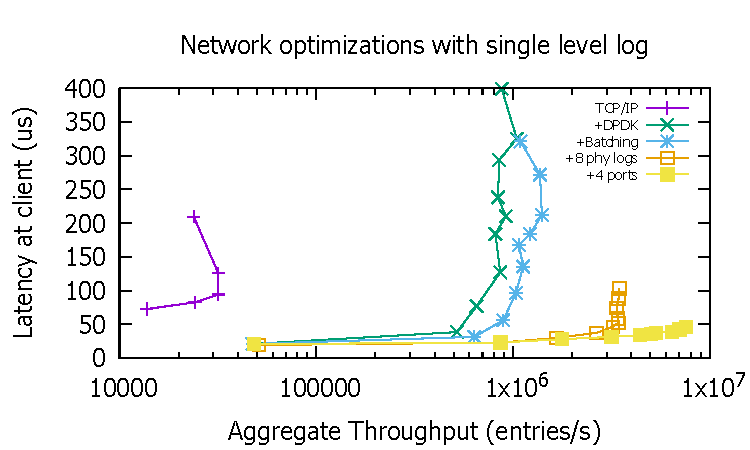
\includegraphics[scale=0.6]{results2/network_opts.pdf}
\caption{Network optimizations for top level log}
\label{fig:network_opts}
\end{figure}

There are two factors that can have significant impact on Cyclone's
performance. First, the number of replicas dictates the outgoing message rate
from the leader replica and therefore increasing the replication factor can
decrease Cyclone's performance. Figure~\ref{fig:replicas} shows the impact of
varying replica count. Using only a single replica cuts out a network round trip
and shows the best unloaded latency (10 us) and peak throughput (near 10M
entries/s). Adding replicas decreases the peak throughput down to around 2M
entries/s with 5 replicas. We note that a number of previous pieces of
work~\cite{faast, farm} use three replicas and therefore we focus on three
replicas for the replicated cases we consider below. The second factor that
dictates Cyclone's performance is the size of the log entry being
replicated. Figure~\ref{fig:payload} shows the effect of increasing the payload
size from zero to 512 bytes. Peak throughput drops from 6M entries/s to
approximately 2M entries/s. At this replication rate, the leader replica needs
to transmit data at approximately 30 Gbit/s. Coupled with the cost of network
headers all four 10 GigE ports are now saturated and therefore Cyclone hits the
network line rate bottleneck at this point.

\begin{figure}
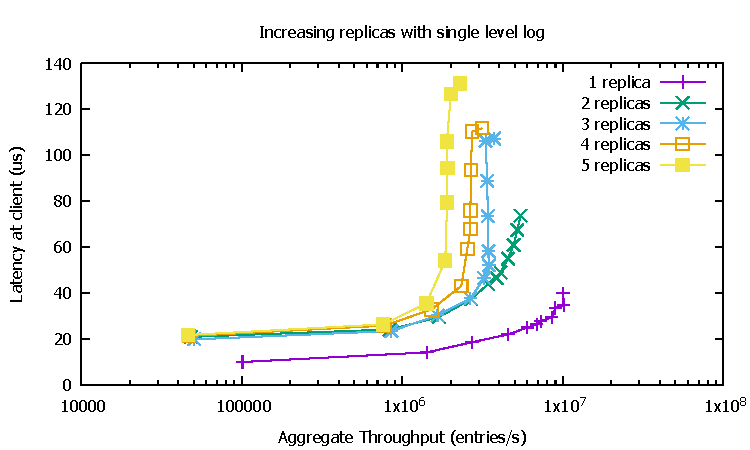
\includegraphics[scale=0.6]{results2/replicas.pdf}
\caption{Impact of replica count}
\label{fig:replicas}
\end{figure}

\begin{figure}
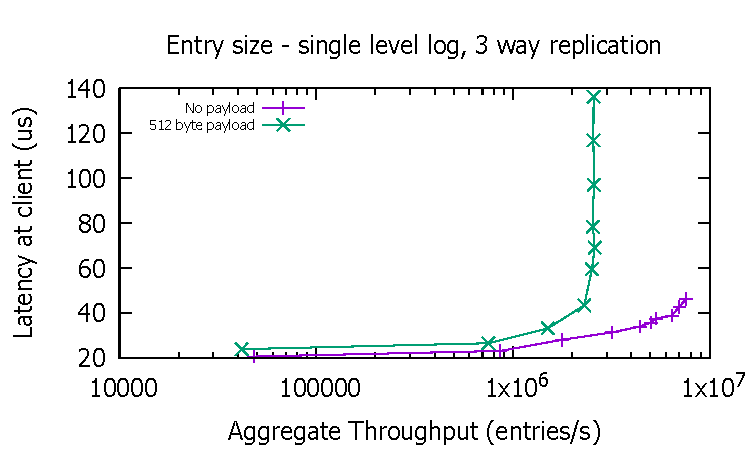
\includegraphics[scale=0.6]{results2/512.pdf}
\caption{Impact of payload size}
\label{fig:payload}
\end{figure}

We now turn our attention from the network component of Cyclone to the storage
one by adding the second level flashlog. We evaluate the impact of adding
block storage to our hitherto pure packet switching scenario in
Figure~\ref{fig:flashlog}. Batching entries from the top level NVDIMM log to the
second level flashlog is clearly beneficial as adding flash storage at the
second level has almost no impact on peak performance in Cyclone for small
entries. The situation however changes for larger
entries. Figure~\ref{fig:flashlog_512} shows that using a 512 byte payload has a
significant impact on peak throughput - it drops to approximately 350K
ops/sec. This corresponds to around 50K 4KB IOPS to the SSD to write out the
flashlog pages. The peak for the drive is 160K IOPS using a queue depth
(concurrency) of 128. With 32 application threads we expect a lower peak
throughput around 40K IOPS explaining our bottleneck at 50K IOPS.  It is
possible to tune our observed performance further by aligning the flush boundary
to increase the number of outstanding requests - we do not do so in this paper,
keeping Cyclone agnostic to the exact size of entry being replicated. A final
point about Figure~\ref{fig:flashlog_512} is that once we are past the storage
bottleneck the latency spike is dramatic and large enough to trigger Cyclone's
failure detector and repeated retries from the clients. There are - therefore -
no points on the ``knee'' of the curve as in the pure packet switched one-level
log case.

\begin{figure}
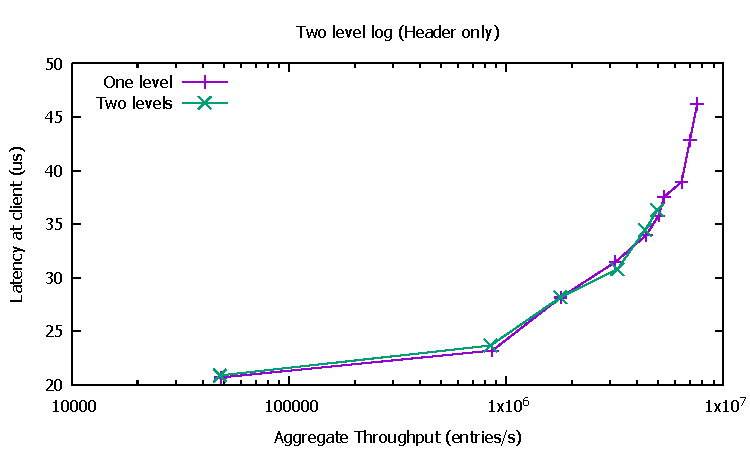
\includegraphics[scale=0.6]{results2/flashlog.pdf}
\caption{Impact of adding second level log}
\label{fig:flashlog}
\end{figure}

\begin{figure}
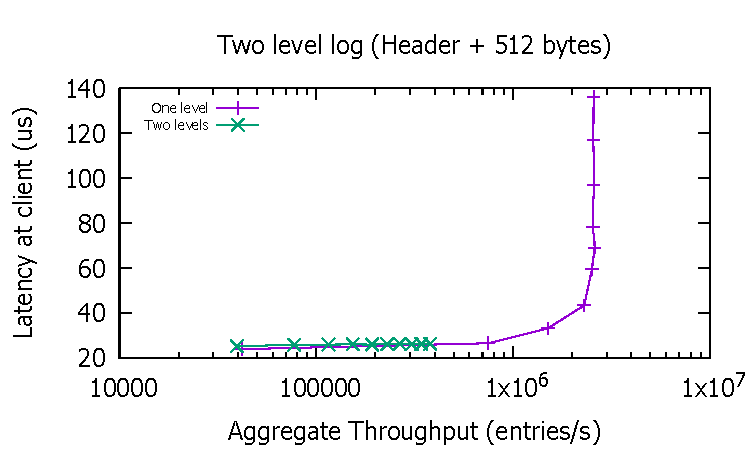
\includegraphics[scale=0.6]{results2/flashlog_512.pdf}
\caption{Second level log with 512 bytes payload}
\label{fig:flashlog_512}
\end{figure}

The final dimension we evaluate is of ganged operations. The primary purpose of
ganged operations is to avoid the need for distributed transactions to
manipulate what is a single shared memory image and therefore we were most
concerned about unloaded latency given the complexity of synchronizing different
replication quorums as well executing our rendezvous protocol on multiple
cores. We therefore setup an experiment where a single client - reflecting the
unloaded case - made ganged requests to the replicas. We varied the number of
cores participating in the request from one to the full complement of 32
application cores. Figure~\ref{fig:ganged} shows the results both using a single
level log as well as a two level log. The primary takeaway is that unloaded
latency increases slowly as we increase the number of active cores - to around
40 us from the baseline of 20 us. There are two causes of this. First, there is
a quicker rate of increase from 1 to 8 active cores, the reason being that this
corresponds to an increase in the number of physical logs that must be
synchronized on. There is some amount of synchronization involved in the
userspace DPDK driver for access to common resources for accessing the NIC and
this affects the ability to simultaneously issue replication messages on all
quorums. The smaller contribution to increasing latency that continues past the
8 core case is due to cacheline pingponging when executing the rendevous of
Figure~\ref{fig:ganged_ops}. Both these sources of latency drift could be
corrected using replication quorums mapped to dedicated NICs and more scalable
rendezvous designs (such as with machine aware broadcast
trees~\cite{broadcast_tree}). However we deemed the complexity of such
optimizations unnecessary. The added latency for most cases is well under the
extra round trip delay (including replication) for all phases of a 2PC.

\begin{figure}
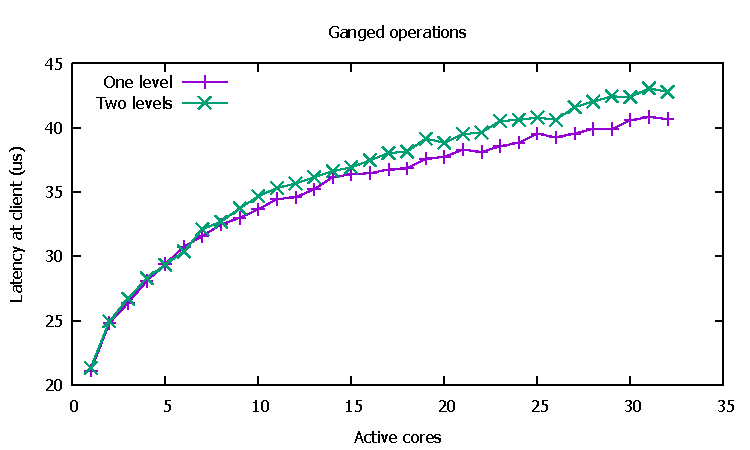
\includegraphics[scale=0.6]{results2/multi.pdf}
\caption{Ganged Operations}
\label{fig:ganged}
\end{figure}

We now evaluate Cyclone integrated with the Rocksdb persistent key value
store. Rocksdb is a complex industrial strength persistent key value store and
this means that it is accompanied by a complex array of performance tuning knobs
to get the best performance from flash. We were also aware that SSD performance
is slated for dramatic increases in the coming years with the introduction of
new memory technology such as 3DXPoint based Optane SSDs. To demonstrate that
Cyclone is future proof we eliminated flash media performance from the picture
as far as the key value store is concerned by placing all files for the key
value store (SSTables) on a RAMdisk, which presumably represents the limit in
performance for flash in the near future. All log files on secondary storage
however - both Rocksdb's own write ahead log and the alternative of Cyclone's
second level flashlog - are placed on the SSDs.

We evaluate two different request sizes: 8 byte keys with 8 byte values and 8
byte keys with 256 byte values. We run 8 physical logs on 8 cores and devote 32
cores to Rocksdb. Since we are interested in performance of the log, which is
only used for update requests, our workload is 100\% writes.

Before evaluating with Rocksdb, we measure the baseline performance of
replicating the log with Cyclone for the given request sizes - Rocksdb performs
a no-op. We note that in addition to the key and value, we are also logging
RocksDB specific request data such as operation type and the request header.
Figure~\ref{fig:kv_baseline} shows the baseline performance for the chosen
request sizes. With the smaller request size, Cyclone can conservatively sustain
close to a million requests a second at a latency of just under 25us. With the
larger request size, Cyclone can sustain around 350K requests a second, again at
a latency of just under 25 us. Armed with these baseline numbers we now examine
how well Cyclone performs with Rocksdb.

\begin{figure}
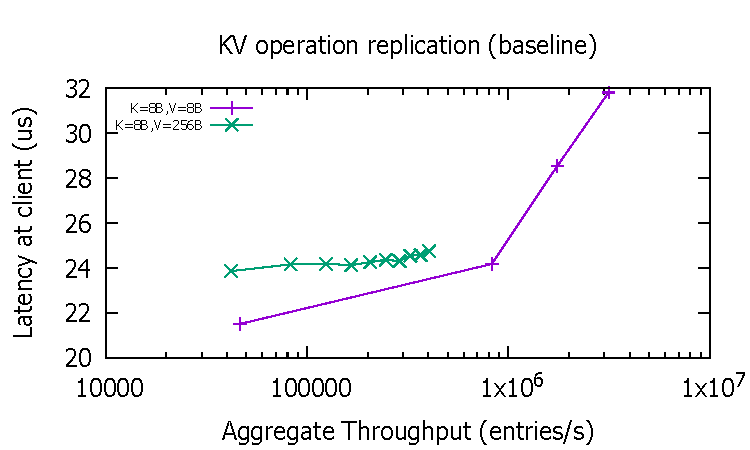
\includegraphics[scale=0.6]{results2/kv_baseline.pdf}
\caption{Baseline KV replication performance}
\label{fig:kv_baseline}
\end{figure}

The performance of Rocksdb with Cyclone for the small update workload is shown
in Figure~\ref{fig:rocksdb} - essentially presenting the solution to the problem
description graph in Figure~\ref{fig:problem}.  We consider four different
setups. The line labeled 'rocksdb' is the key value store running with no
logging whatsover - a system crash would lead to data loss. The line labeled
'rocksdb/wal' is for Rocksdb running with its write ahead logging turned on. The
large gap between these two is the overhead of the existing Rocksdb WAL
solution. The line labeled 'rocksdb/Cyclone 1 way' is a two level Cyclone log
but without any replication. The line almost exactly tracks the performance of
Rockdb. As suggested by the baseline replication performance, Cyclone is able to
provide a write ahead log with no overhead to Rocksdb. The line labeled
'rocksdb/Cyclone 3 way' is with 3-way replication turned on. Other than a 20us
delta due to the extra network round trip, the line almost exactly tracks
Rocksdb performance with no logging. Cyclone therefore provides high
availability to Rocksdb at a fraction of the cost of its existing single machine
write ahead log. We also repeat the experiment for the larger update size in
Figure~\ref{fig:rocksdb_256}. The conclusions are identical: Cyclone solves
Rocksdb's write ahead logging problem.

\begin{figure}
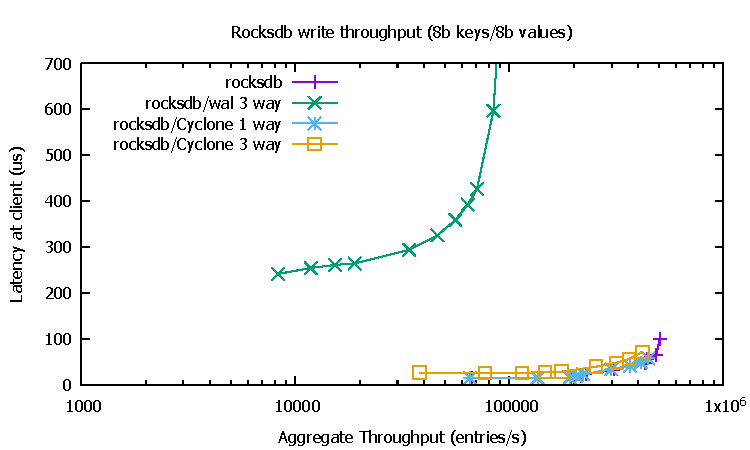
\includegraphics[scale=0.6]{results2/rocksdb.pdf}
\caption{Rocksdb - small updates}
\label{fig:rocksdb}
\end{figure}

\begin{figure}
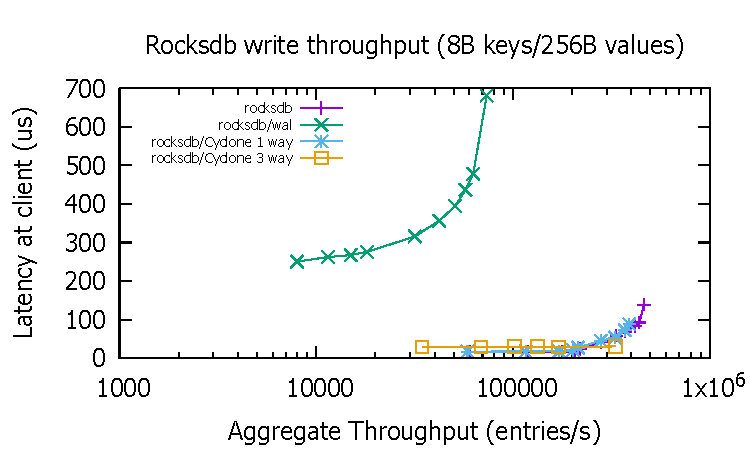
\includegraphics[scale=0.6]{results2/rocksdb_256.pdf}
\caption{Rocksdb - large updates}
\label{fig:rocksdb_256}
\end{figure}

Next, we consider the problem of supporting Rocksdb's write-batch operation that
atomically writes a set of key-value pairs into the KV store. In order to
perform the operation with Cyclone managing the log, the client must issue a
ganged operation across cores owning the keys in the write batch. This is in
contrast to baseline Rocksdb where the entire write batch can be sent to any
core. A key concern here was whether Cyclone would add any latency to the
operation due to the extra synchronization needed across replication quorums and
participating application cores. We examine the problem for the unloaded case
and small updates in Figure~\ref{fig:rocksdb_multi} for a single client with
increasing number of keys in the batch - till 32 keys that covers all
application cores. The line labeled Rocksdb is with no write ahead logging. We
note an increasing latency for this baseline indicating Rocksdb takes longer
with larger key batches. The existing option of Rocksdb/wal has considerably
larger latency. Cyclone does an effective job of cutting down on this latency
even as it needs to pay a price for synchronizing multiple quorums and
application cores making it somewhat slower than running Rocksdb with no logging
for batched writes. A distributed 2PC transaction still remains more expensive
just in terms of network delay than using Cyclone.

\begin{figure}
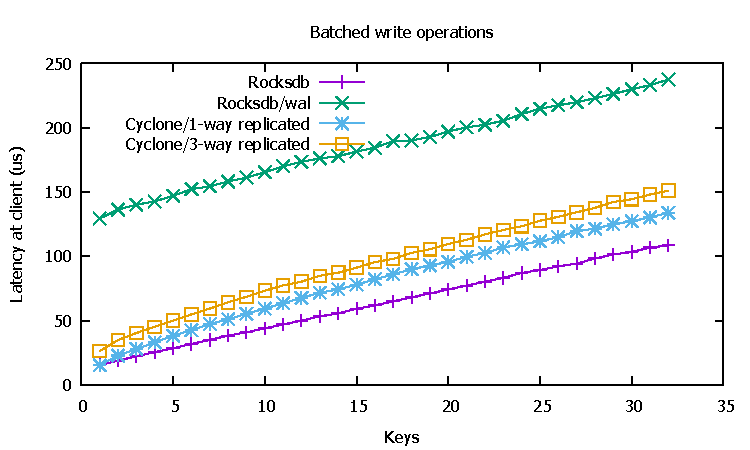
\includegraphics[scale=0.6]{results2/rocksdb_multi.pdf}
\caption{Rocksdb - batched writes}
\label{fig:rocksdb_multi}
\end{figure}

Finally, we showcase the benefit of using Cyclone beyond pure performance as
compared to the existing single machine Rocksdb write ahead log. Cyclone brings
multi-machine availability with the ability to automatically failover. We
demonstrate this in Figure ~\ref{fig:timeline} that shows the timeline of a run
where we kill the server process on the leader replica. Cyclone is configured to
with a 30ms failure detection timeout after which the client library tries
replicas in turn to locate the leader - in this case it fails over in about
60ms.

\begin{figure}
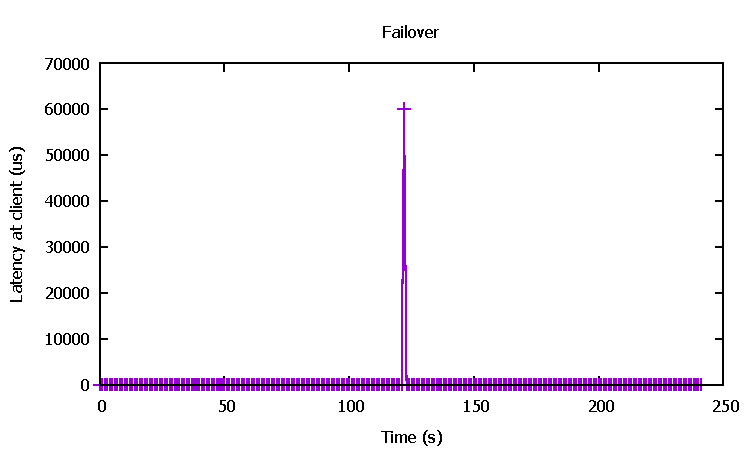
\includegraphics[scale=0.6]{results2/failover.pdf}
\caption{Rocksdb - failover}
\label{fig:timeline}
\end{figure}

\section{Related Work}

Cyclone takes a software only approach to improving replication performance
using commodity network hardware. In contrast, Mojim~\cite{mojim} pairs directly
attached persistent memory with RDMA to replicate persistent data structures. On
40Gbps infiniband, Mojim reported being able to mirror data at 4GB/s. In
contrast, Cyclone can replicate data three ways using 4*10 Gbps commodity
ethernet NICs at a peak of roughly 3.7 GB/s. Notably this is while Cyclone is
also running the RAFT consensus protocol and draining the log to a high capacity
flash SSD, while Mojim is doing simple mirroring of main memory. One can
conclude that network offload via RDMA and Infiniband is not an a-priori
requirement for high throughput replication. This is made possible by Cyclone's
approach that relieves the CPU from the burden of data copies. Of course, the
latency of a hop on commodity ethernet at 5 us with our DPDK stack is larger
than the close to 2us latency with Infiniband. Depending on the use case for the
key value store application the extra 6us with ethernet for the round trip to
the replica might be a concern for some applications. We note that mapping the
commutativity of key value store interfaces to multiple logs in Cyclone is a
technique that can also be applied to RDMA. The authors of Mojim confirm that
concurrency is a significant determinant of performance when replicating over
RDMA.

Consensus in a box~\cite{consensus_box} implements the Zookeeper atomic
broadcast protocol together with a NIC on an FPGA. That work ignored durability,
focusing purely on network performance for replication. Latency numbers are
excellent due to the FPGA that cuts out the path from CPU caches to the NIC and
are reported to be as low as 3us for a round trip from leader to follower
replica compared to the 6us we observe with DPDK. Notably however they reported
7us when using TCP/IP from the FPGA rather than their own connection oriented
network protocol. On the other hand their peak replication throughput is 6M
replications/sec on 66 Gbps of aggregate network bandwith, comparable to the
same mark obtained by Cyclone on an aggregate 40 Gbps of network bandwidth. We
believe the general applicability afforded by our software only solution
together with the fact that we provide persistence by design makes it a
compelling alternative to an FPGA based solution even given the larger latency.

{CRANE}~\cite{crane} is a system for replicating mutithreaded programs using
Paxos. It uses deterministic multi-threading to ensure replicas converge to the
same state as opposed to semantic equivalence in Cyclone using the commutativity
of the key value store interface. Although CRANE is more generally applicable in
that it makes no assumptions about the application API, deterministic
multithreading comes with high overheads for applications that store large
amounts of data - CRANE reports around a 2X slowdown for MySQL, likely rendering
it unsuitable as a replacement for the write ahead log in key value stores.

The scalable commutativity rule~\cite{scalable_commutativity} generalizes the
idea of commutativity in key value store interfaces that we have used for
horizontal scaling in Cyclone. Conveniently, it provides a tool for checking when
API calls can commute in a history. It is a simple exercise to express a key
value store API in COMMUTER and check that operations to different keys
commute. This provides a theoretical basis for horizontal scaling, something we
have omitted for brevity from this paper. The scalable commutativity rule also
suggests that scalable key value store implementations would necessarily have
commutative interfaces, something we confirm and exploit for key
value stores.

There is an in progress transformation of durable memory in datacenters
with the advents of 3DXPoint. Researchers have speculated on the impact of cheap
and high volume directly attached 3DXPoint~\cite{tiering}. Memory vendors have
also begun shipping software libraries such as NVML~\cite{nvml} for building durable
in-memory data structures using undo logging. A durable key value store using
3DXPoint would be an idea target for Cyclone because each NVM log entry can be
discarded as soon as it is applied to the persistent key value store removing
the need for the flashlog. This would allow Cyclone to operate at pure packet
switching speeds, a goal we hope to achieve in the future with a single level
log for NVML data store applications.

Cyclone provides a client library that automatically times out and retries
requests to deal with failure. Protection against repeated execution of the same
request is currently left to the key value store and client, since we felt that
exactly once semantics is optional when updates such as put operations are
idempotent. We have experimented with exactly once semantics as a basis for
distributed transactions across shards running Cyclone integrated key value
stores, along the lines of similar work~\cite{raft_lin}, using a fixed client
space and maintaining information about last seen sequence numbers from clients
in NVM. Distributed transactions on Cyclone shards however are outside the scope
of this paper.

\section{Conclusion}
Persistent key value stores struggle today to provide high availability using a
write ahead log without a significant impact to performance. Cyclone solves this
problem by leveraging a small amount of directly attached non-volatile memory
that transforms the replication problem into a software packet switching
problem. Cyclone and its Rocksdb bindings are slated for release to the open
source community and we hope both the code and the ideas in the system itself
will help key value store builders and researchers overcome their logging
problem.
\newcommand\myurl[2]{\url{#1}}
\bibliographystyle{plain}
\bibliography{paper}

\end{document}



